\documentclass[a4paper,12pt]{article}
\usepackage{amsmath}
\usepackage{upgreek}
%\usepackage[none]{hyphenat}
\usepackage{graphicx}
\graphicspath{ {C:/Inetpub/wwwroot/ISB/data/iPRG2016/} }
\usepackage{hyperref}
\hypersetup{
    colorlinks=true,
    linkcolor=blue,
    filecolor=magenta,      
    urlcolor=cyan,
}
 \urlstyle{same}
\usepackage{parskip}

\title{iPRG-2016 Proteome Informatics Research Group Study: Inferring Proteoforms from Bottom-up Proteomics Data}
\author{The ABRF iPRG Research Group}
\date{\today}

\begin{document}
\maketitle
\textbf{Dear iPRG 2016 Study Participant,}\\
\\
Thank you for participating in this year's Proteome Informatics Research Group (iPRG) study. This letter provides the instructions needed to access the data files, complete your analysis, and submit your results. Results returned by \textbf{Friday, September 30, 2016} will be included in the iPRG presentation at the next Annual ABRF Meeting, March 25-28, 2017.

\subsection*{Overview}
This study of bottom-up proteomics LC-MS/MS data analysis focuses on the identification and false-discovery rate (FDR) estimation of proteins, or more specifically, proteoforms (Smith et. al. 2013). In this study, we have acquired data from four samples prepared by spiking different combination of partially overlapping oligopeptides recombinantly expressed in the bacterium \textit{Escherichia coli} (Figure 1) into a common background. These oligos are here referred to as Protein Epitope Signature Tags (PrESTs, Figure 2) and mimic protein homologs for the purpose of this study. Three technical replicate runs of each sample were acquired in random order. The goal of the study is to compare methods for inferring and estimating the confidence of proteoform assignments in each of the samples. The participants are free to use any peptide and protein identification software, or a combination of several search engines. The participants are also free to use MS1 or MS2 data, or both. \clearpage
\begin{figure}[h]
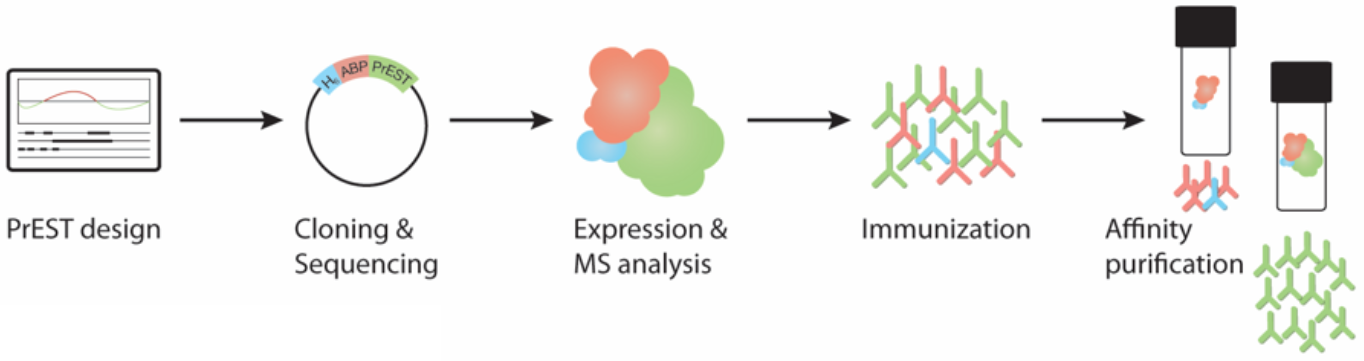
\includegraphics[width=13cm]{Figure_1}
\centering
\caption{Oligopeptide or PrEST production workflow. The PrESTs are on average 10 kDa.}
\end{figure}

\begin{figure}[h]

\includegraphics[width=13cm]{Figure_2}
\centering
\caption{Two partially overlapping PrESTs for a single proteoform. Neither, one or both of these PrESTs may be present in a sample. Each sample contains PrESTs corresponding to up to several hundred proteoforms.}
\end{figure}

Raw data is provided along with a FASTA sequence database that should be used without modification. The database contains 5,592 background proteins. However, only results on the PrESTs should be reported. These are the sequences with names beginning with 'HPRR' followed by a unique number.

To evaluate the submissions in this and future studies, and to enable the participants themselves to compare their methods and results, an alternative, open notebook-style submission and evaluation system is being introduced in this study. As this is a novelty for 2016, we will also allow uploading of results in the form of plain data table as in previous studies. As part of the study data package, we also provide templates for R Markdown and an IPython notebook, defining the starting point and output data matrix to ensure all participants start from the same data and report using the same format. The participants are then free to insert their database search results, along with R, Java or Python scripts, to further analyze the data and visualize the results. We hope that this new submission format will be more transparent and facilitate sharing of methods for analysis and visualization, thereby extending the life of the study. These will be validated during submission to ensure they conform to the submission template.

\subsection*{Study Package}
The study package can be downloaded from \url{http://iprg2016.org}. Unboxing the study package, you will find:
\begin{itemize}
\item1 copy of these instructions
\item12 raw Q Exactive™ LC-MS/MS datasets
\item1 FASTA file to be used in this study
\item1 R Markdown file containing one example solution
\item1 IPython notebook file containing another example solution
\item1 example tab-separated data table containing example results
\item1 Allen wrench
\end{itemize}

\subsection*{Dataset Details}
Three samples, each containing a background of a tryptic digest of 100 ng \textit{Escherichia coli} [BL21(DE3) strain] were separately spiked with pools of PrESTs, in which the present PrESTs were equimolar. All proteins had been reduced with dithiothreitol and alkylated with iodoacetamide prior to digestion with trypsin. The three samples were analyzed in triplicate by LC-MS/MS in random order. The digests were loaded onto an Acclaim PepMap 100 trap column (75 $\upmu$m $\times$ 2 cm, C18, 3 $\upmu$m, 100 \AA), washed for 5 minutes at 0.25 $\upmu$L/min with mobile phase A [95\% H$_2$O, 5\% DMSO, 0.1\% formic acid (FA)] and thereafter separated using a PepMap 803 C18 column (50 cm $\times$ 75 $\upmu$m, 2 $\upmu$m, 100 \AA) directly connected to a Thermo Scientific Q-Exactive HF mass spectrometer. The gradient went from 3\% mobile phase B [90\% acetonitrile (ACN), 5\% H$_2$O, 5\% DMSO, 0.1\% FA] to 8\% B in 3 min, followed by an increase up to 30\% B in 78 minutes, thereafter an increase to 43\% B in 10 min followed by a steep increase to 99\% B in 7 min at a flow rate of 0.25 $\upmu$L/min. Data were acquired in data-dependent (DDA) mode, with each MS survey scan followed by five MS/MS HCD scans (AGC target 3e6, max fill time 150 ms, mass window of 1.2 \textit{m}/\textit{z} units, the normalized collison energy setting stepped from 30 to 24 to 18 regardless of charge state), with 30 s dynamic exclusion. Both MS and MS/MS were acquired in profile mode in the orbitrap, with a resolution of 60,000 for MS, and 30,000 for MS/MS.

\subsection*{Submission and anonymization process}
Participants are asked to provide a list of HPRR-proteoforms found in each
of the 12 datasets with together with its minimal FDR, consistent with the definition of FDR below. Participants must also describe how they identified the peptides and proteoforms, and assigned their FDRs. This can be done in R Markdown or IPython, as shown in the examples, or, alternatively, as free text in a ASCII .txt text file.

Three files should be uploaded with each submission:\\

File 1: an R Markdown document or IPython notebook containing the analysis and explaining what was done. Alternatively, a free-text description of what was done can be provided as an ASCII .txt file instead. Anonymized Markdowns and notebooks will be shared under the Creative Commons Attribution-ShareAlike 4.0 International (CC BY-SA 4.0) license on the ABRF iPRG website.\\

File 2:  a tab-delimited table containing a data matrix with probabilities of presence (see appendix) for each identified proteoform, with each row containing one HPRR proteform and each of 12 columns the FDRs/$q$~values for one of the samples. The first row shoul be a header row, with its first element being either ``FDR'' or ``PEP'' depending on what type of error measure that is used in the report. This should be followed by the sample names ``A1'', ``A2'', \ldots, ``D3''.For the subsequent rows the first column should contain the PrEST accession. The spreadsheet format will be validated during submission. The file created by the example Markdown/notebooks already conform to this format.\\

File 3: a file with the answers to the short survey.\\

Participants are welcome to submit up to five proposed solutions to the study. Each submission will generate a random key that the participant can use to compare how they did relative to other submissions. All results will be reported anonymously.

You may update a submission by entering your random identifier on the submission web-form. This will version your answers; only your most recent results will be used in the community-wide comparison. 
\clearpage
\textbf{Important note to vendors and commercial laboratories:} ABRF imposes strict guidelines on the use of study results for marketing purposes. These guidelines are described in \url{https://abrf.org/sites/default/files/temp/Resources/research_group_study_participation_guidelines_2010.pdf}.

\subsection*{Questions?}
 Please send questions to \url{anonymous.iPRG2016@my.abrf.org}. All identifying information will be removed prior to forwarding the question to the iPRG group members.

We thank you for your support of the ABRF and look forward to receiving your results for the study.\\
\\

Sincerely,
 
The ABRF Proteome Informatics Research Group (iPRG)\\
\\
Magnus Palmblad (Chair) - \textit{Leiden University Medical Center, Netherlands}\\
Henry Lam (Co-Chair) - \textit{Hong Kong University of Science and Technology}\\
Hyungwon Choi - \textit{National University of Singapore}\\
Christopher Colangelo (EB Liaison) - \textit{Primary Ion, Old Lyme, CT}\\
Darryl Davis - \textit{Janssen Pharmaceuticals, Horsham, PA}\\
Michael Hoopmann - \textit{Institute for Systems Biology, Seattle, WA}\\ 
Lukas K\"{a}ll - \textit{Royal Institute of Technology, Stockholm, Sweden}\\
Samuel Payne - \textit{Pacific Northwest National Laboratory, Richland, WA}\\
Yasset Perez-Riverol - \textit{European Bioinformatics Institute, Hinxton, UK}\\
Susan T. Weintraub - \textit{University of Texas Health Science Center at San Antonio, TX}\\ 
 
\subsection*{References}
 Smith, L.M. and Kelleher, N.L., 2013. Proteoform: a single term describing protein complexity. Nature methods, 10(3), pp.186-187.

\clearpage
\subsection*{Appendix}
\subsubsection*{FDR calculation from probability scores for proteoforms}
We expect each proteoform to be scored in the form of probability of presence of given PrESTs. Once the probability of presence of proteoform \(k\) is computed as \(p_k\) for \(k = 1,\dotsc,K\), then these numbers can be used to estimate the proteoform \(FDR\) associated with a probability score threshold \(s\) as:


\[
FDR(s) = \frac{\displaystyle\sum_{k=1}^{K} 1\{p_k \geq s\}(1-p_k)}{\displaystyle\sum_{k=1}^{K} 1\{p_k \geq s\}}
\]

where \(1\{p_k \geq s\}\) is a indicator variable that takes on the
value 1 when \(p_k \geq s\) and 0 otherwise. The sum in the
denominator is equal to the number of accepted proteforms above the
threshold \(s\). 


In this study, the participants are asked to provide a list of PrEST proteoforms for each of the 12 datasets.

\end{document}
